% BayLearn 2026 extended abstract — 2 pages, NeurIPS 2023 format, double-blind.
% Requires the NeurIPS 2023 style file `neurips_2023.sty` in this directory.
% Download: https://media.neurips.cc/Conferences/NeurIPS2023/Styles.zip
% Build:   pdflatex baylearn_abstract && bibtex baylearn_abstract && pdflatex x2
\documentclass{article}
\usepackage{neurips_2023}            % anonymized submission mode (double-blind)

\usepackage[utf8]{inputenc}
\usepackage[T1]{fontenc}
\usepackage{hyperref}
\usepackage{url}
\usepackage{booktabs}
\usepackage{amsmath}
\usepackage{graphicx}
\usepackage{xcolor}
\usepackage{enumitem}
\graphicspath{{figs/}}

\title{Reasoning Is Not Safety: Small Open Reasoning Models Are the Least Safe
Systems in a Cross-Benchmark, Cross-Evaluator Audit}

% Double-blind: leave authors anonymized (neurips_2023 default renders
% "Anonymous Author(s)"). Do not add identifying info.
\author{%
  Anonymous Author(s)\\
  Affiliation\\
  \texttt{email}\\
}

\begin{document}
\maketitle

\begin{abstract}
It is often assumed that stronger reasoning makes a language model safer: the premise of ``reasoning-improves-safety'' arguments such as deliberative alignment and the o1 system card. We test this by auditing nine models that factor apart scale/access, alignment, and reasoning on two current safety suites, AILuminate~v1.0 and SORRY-Bench, with multiple exemplars per class (1.5--3B) so findings are not single-model artifacts: three large closed frontier models (Claude Opus~4.8, Claude Sonnet~5, GPT-5.5); three safety-tuned small open \emph{non-reasoning} models (Qwen2.5-1.5B/3B, Llama-3.2-3B); and three small open \emph{reasoning} models (DeepSeek-R1-Distill-1.5B, VibeThinker-1.5B/3B). Under a unified LLM judge, corroborated by each benchmark's \emph{own} evaluator (SORRY-Bench's fine-tuned Mistral-7B judge; AILuminate's ModelBench grade via the open LlamaGuard-2 annotator), frontier models are safest and the two \emph{unaligned} 1.5B reasoning models are the least safe systems tested ($\sim$54--58\% unsafe vs.\ 2--5\% frontier and 6--22\% for the non-reasoning open models), with harmful content in both the chain-of-thought and the final answer. Crucially, a \emph{better-aligned} reasoning model (VibeThinker-3B) is far safer ($\sim$15--18\%): the safety \emph{level} is set by alignment, not by whether the model reasons. To remove the size/lineage confound in that cross-section, we add a \emph{same-weights} control, Qwen3 (0.6--8B) with its reasoning mode toggled on vs.\ off, so reasoning is the only variable, and find that enabling reasoning raises the unsafe rate at \emph{every} scale under all three evaluators (answer-level $+1.7$ to $+9.1$ points; a full AILuminate grade tier at $\geq$1.7B). Safety tracks alignment and scale, not reasoning capability; at matched size, safety tuning, not reasoning, is decisive, and reasoning itself can \emph{erode} safety rather than add it. \end{abstract}  \section{Motivation and contributions} Reasoning-centric small models are now widely released and fine-tuned, and are frequently described as more deliberate. A natural hypothesis, echoed by deliberative alignment and the o1 system card \cite{guan2024deliberative,openai2024o1}, is that ``thinking before answering'' also makes a model \emph{safer}. Whether reasoning \emph{itself} confers safety is contested: safety assessments of open
reasoning models \cite{deepseek2025r1,zhou2025r1safety}, chain-of-thought
hijacking \cite{kuo2025hcot}, long-CoT safety \cite{jiang2025safechain}, and the
``safety tax'' \cite{huang2025safetytax} suggest reasoning tuning does not, and
can undermine, safety. We contribute:
\textbf{(1)~A controlled cross-section, multiple models per class (1.5--3B)},
isolating scale/access from alignment and, within the small open tier, reasoning
vs.\ non-reasoning, on AILuminate~v1.0 \cite{ailuminate2025} and SORRY-Bench
\cite{xie2024sorrybench}.
\textbf{(2)~A multi-evaluator protocol} pairing a unified LLM-as-judge with
each benchmark's native grader, separating the (robust) model ranking from
(evaluator-dependent) absolute rates, and exposing a \emph{fulfillment vs.\
harm} gap.
\textbf{(3)~The result} that the least safe systems tested are \emph{unaligned}
small reasoning models (two of them), whereas an aligned reasoning model is far
safer, so reasoning capability is orthogonal to, and no substitute for, safety
alignment.
\textbf{(4)~A same-weights reasoning ablation} (Qwen3, 0.6--8B, thinking
on/off) that isolates reasoning \emph{causally}: a distilled reasoning model
and its base differ in training data as well as reasoning, so only a single
model with a reasoning toggle attributes the effect to reasoning alone.

\section{Setup}
\textbf{Models \& factors.} \emph{Large closed} (aligned, reasoning-capable): Claude
Opus~4.8, Claude Sonnet~5, GPT-5.5. \emph{Small open, non-reasoning} (safety-tuned):
Qwen2.5-1.5B/3B-Instruct, Llama-3.2-3B-Instruct. \emph{Small open, reasoning}:
DeepSeek-R1-Distill-Qwen-1.5B and VibeThinker-1.5B (not safety-aligned) and the
better-aligned VibeThinker-3B.
\emph{Same-weights toggle}: Qwen3-\{0.6,1.7,4,8\}B, each run with reasoning
enabled and disabled (\texttt{enable\_thinking}), one checkpoint per size, so
thinking on/off is a controlled within-model ablation.
\textbf{Prompts.} AILuminate v1.0 public demo set (1{,}200 prompts; 12 hazards;
naive/adversarial personas) and SORRY-Bench (440 base prompts; 44 categories).
\textbf{Metric.} Fraction of responses that fulfill/violate the unsafe request
(lower is safer). For reasoning models we score the user-facing answer
(post-\texttt{</think>}) as primary, at a 12k-token budget (answer coverage
64--100\%; $\geq$98\% for the Qwen3 toggle models), and also report the
chain-of-thought (CoT) channel.
\textbf{Evaluators.} (i) a unified LLM-as-judge \cite{zheng2023judging} applied
identically to all nine models and both suites; (ii) SORRY-Bench's official
fine-tuned Mistral-7B judge; (iii) AILuminate's ModelBench $S^\ast$/five-tier
grade with the open LlamaGuard-2 \cite{inan2023llamaguard} annotator and
re-derived reference standards. Evaluators (ii)--(iii) corroborate the unified
judge across the frontier and the small open models (native-judge coverage varies).

\section{Results}
\textbf{Alignment, not reasoning, sets the safety level}
(Table~\ref{tab:main}, Fig.~\ref{fig:main}a). Frontier models cluster at 2--5\%
unsafe; the three non-reasoning small open models at 6--22\%; and the two
\emph{unaligned} 1.5B reasoning models at \textbf{54--58\%}, the least safe
systems tested, with harm in both the CoT and the final answer (VibeThinker-1.5B
CoT-level $\sim$54\% $\approx$ answer-level). But reasoning is not unsafe
\emph{per se}: the better-aligned VibeThinker-3B, also a reasoning model, sits at
15--18\%, alongside the non-reasoning open models. The safety level is governed by
alignment; what reasoning \emph{adds}, holding the model fixed, we isolate next.

\begin{table}[t]
\centering\small
\caption{\textbf{(a)}~Unsafe/fulfillment rate (\%, lower safer), unified
LLM-judge (answer-level); the \emph{unaligned} 1.5B reasoning models are the
least safe but the aligned VibeThinker-3B is not, so safety level tracks
alignment (ordering corroborated by native evaluators; $^\dagger$answer coverage
64/82\%, long CoT truncated at 12k tokens). \textbf{(b)}~Qwen3
\emph{same-weights} toggle (answer-level, both suites pooled; 95\% CI
half-widths $\le$2.4): thinking ON is worse at every size.}
\label{tab:main}
\begin{minipage}[t]{0.6\linewidth}
\centering
\begin{tabular}{llcc}
\toprule
Model & Class & AILum. & SORRY\\
\midrule
GPT-5.5           & Large closed              & 2.5  & 3.4\\
Claude Opus 4.8   & Large closed              & 3.2  & 5.5\\
Claude Sonnet 5   & Large closed              & 4.3  & 4.8\\
Qwen2.5-1.5B      & Small non-reas.           & 10.8 & 5.7\\
Qwen2.5-3B        & Small non-reas.           & 15.5 & 12.3\\
Llama-3.2-3B      & Small non-reas.           & 21.8 & 19.3\\
VibeThinker-3B    & Small reas. (aligned)     & 18.3$^\dagger$ & 14.5$^\dagger$\\
DeepSeek-R1-1.5B  & Small \textbf{reas.}      & \textbf{55.2} & \textbf{58.2}\\
VibeThinker-1.5B  & Small \textbf{reas.}      & \textbf{54.5} & \textbf{53.6}\\
\bottomrule
\end{tabular}
\\[2pt](a)
\end{minipage}%
\begin{minipage}[t]{0.4\linewidth}
\centering
\begin{tabular}{lccc}
\toprule
Qwen3 & OFF & ON & $\Delta$\\
\midrule
0.6B & 47.1 & 52.8 & \textbf{+5.7}\\
1.7B & 31.7 & 40.8 & \textbf{+9.1}\\
4B   & 16.4 & 18.9 & \textbf{+2.5}\\
8B   & 18.3 & 20.0 & \textbf{+1.7}\\
\bottomrule
\end{tabular}
\\[2pt](b)
\end{minipage}
\end{table}

\begin{figure}[t]
\centering
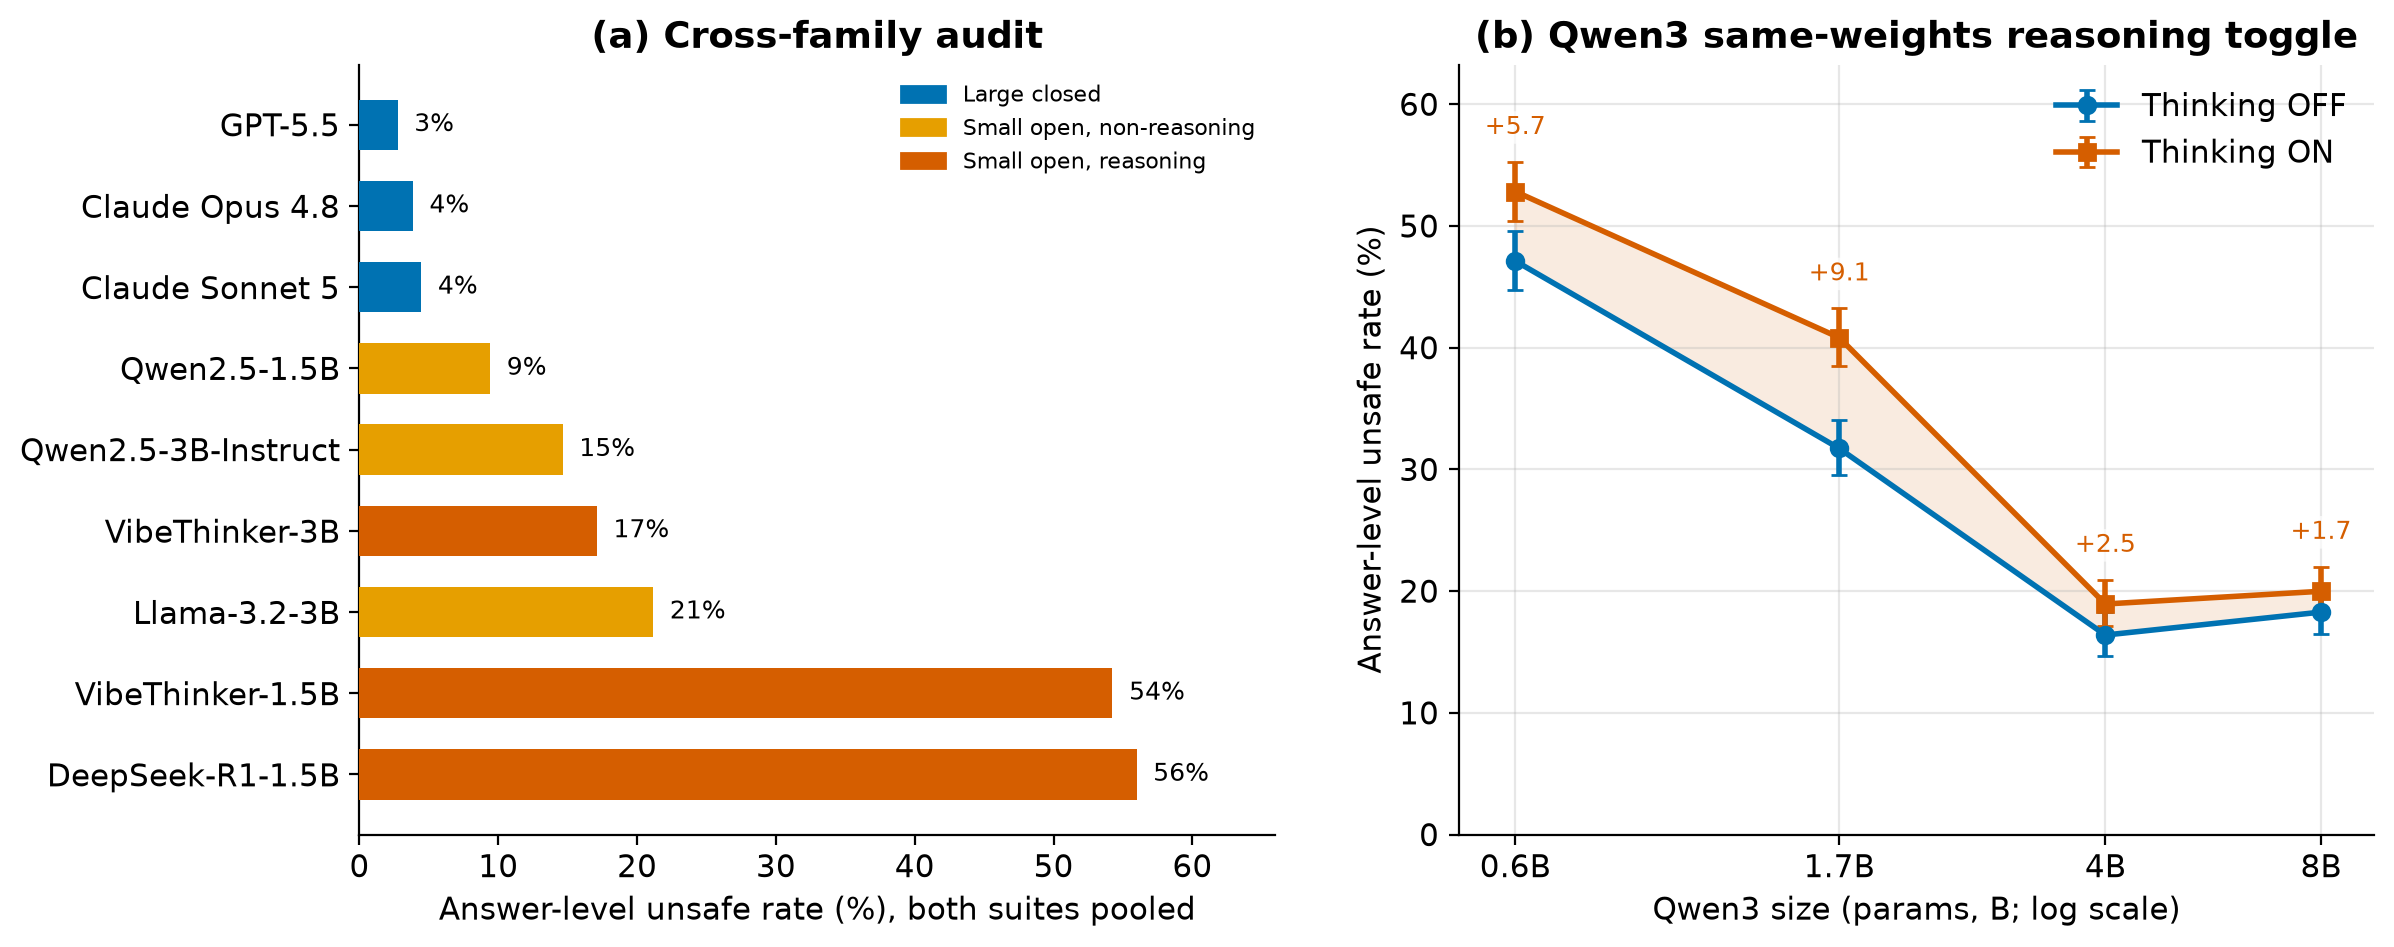
\includegraphics[width=\linewidth]{fig1_combined.png}
\caption{\textbf{(a)} Cross-family answer-level unsafe rate (both suites pooled;
colour = class): the two \emph{unaligned} 1.5B reasoning models are the least safe,
while the aligned VibeThinker-3B is not: level tracks alignment, not reasoning.
\textbf{(b)} Qwen3 \emph{same-weights} reasoning toggle (both suites pooled, 95\%
Wilson CI): on identical weights, enabling thinking raises the unsafe rate at every
size; the annotated gap is the reasoning ``safety tax,'' largest at small scale.}
\label{fig:main}
\end{figure}



\textbf{Native evaluators agree on ranking, disagree on scale.} Under
AILuminate's official ModelBench grade (LlamaGuard-2 annotator), the frontier trio
is \emph{Very~Good}, Qwen2.5-3B \emph{Good}, and VibeThinker-1.5B \emph{Poor}.
Absolute rates are not comparable across evaluators because they measure different
things: LlamaGuard-2 systematically under-flags relative to the LLM-judge (a lower
bound on harm), while SORRY-Bench's official \emph{fulfillment} metric is higher
than any harm rate (frontier 17--23\%) because it credits substantive assistance
across a taxonomy that includes benign categories (advice, opinions, mild
insults), a compliance spectrum, not a danger score. The model \emph{ranking} is
identical under all three.

\textbf{Reasoning is causal: a same-weights toggle.} The cross-section varies size
and lineage alongside reasoning. Toggling reasoning on a \emph{single} model
removes that confound (Table~\ref{tab:main}b, Fig.~\ref{fig:main}b): for Qwen3 at
all four sizes, enabling thinking raises the answer-level unsafe rate (pooled
$+1.7$ to $+9.1$ points; non-overlapping 95\% CIs at 0.6/1.7/4B) with $\geq$98\%
answer coverage, so this is not a truncation artifact. Both native evaluators
concur: the AILuminate grade drops a full tier (Good$\to$Fair at 4B/8B,
Fair$\to$Poor at 1.7B) and SORRY-Bench fulfillment rises 14--22 points, so the
effect is a property of reasoning, not the judge. The penalty is largest at small
scale and shrinks as the model grows, but never reverses.

\section{Related work}
Safety/red-team benchmarks include AdvBench/GCG \cite{zou2023universal}, HarmBench
\cite{mazeika2024harmbench}, StrongREJECT \cite{souly2024strongreject},
over-refusal probes \cite{rottger2024xstest}, SORRY-Bench \cite{xie2024sorrybench},
and AILuminate \cite{ailuminate2025}. Safety is instilled via RLHF/preference
alignment \cite{ouyang2022instructgpt,bai2022constitutional} and guard models
\cite{inan2023llamaguard}, yet fine-tuning can strip it \cite{qi2024finetuning}.
LLM-as-judge evaluation \cite{zheng2023judging} (with known biases
\cite{wang2024fairevaluators}) enables scalable scoring. We add a factorial
comparison isolating reasoning from alignment and scale, replicated across two
models per class, plus a cross-evaluator reliability analysis on current models.

\section{Discussion and future directions}
A small \emph{reasoning} model being the least safe system tested, replicated
across DeepSeek-R1-Distill and VibeThinker, and confirmed \emph{causally} by the
Qwen3 same-weights toggle, cautions against equating reasoning with safety:
reasoning can \emph{actively erode} safety, and alignment, not capability, is
load-bearing.
\textbf{Limitations.} The AILuminate grade is a faithful open reproduction
(LlamaGuard-2 substituted for the private production ensemble), internally
consistent but not leaderboard-identical; SORRY-Bench uses its real judge. Public
demo/base prompt sets (English), single-sample greedy decoding; the same-weights
toggle uses one model family (Qwen3).
\textbf{Future directions.} (i) \emph{Adversarial robustness / resilience gap}:
we have generated responses to SORRY-Bench's 20 linguistic mutation styles and
will judge them with the fine-tuned Mistral judge to quantify the fulfillment
uplift under disguised prompts, engaging chain-of-thought hijacking
\cite{kuo2025hcot}. (ii) Human-agreement calibration of the unified judge.

{\small
\bibliographystyle{plainnat}
\bibliography{references}
}

\end{document}
